% -------------------------------- PREAMBLE --------------------------------
\documentclass[a4paper]{report}

\usepackage[utf8]{inputenc}
\usepackage[T2A,OT1]{fontenc}
\usepackage[english]{babel}
\usepackage{graphicx}
\usepackage{tikz}
\usepackage{booktabs}
\usepackage[format=hang,font=small,labelfont=bf]{caption}
\usepackage[protrusion=true,expansion=true]{microtype}
\usepackage{amsmath}
\usepackage{amssymb}
\usepackage{amsthm}
\usepackage{upgreek}
\usepackage{nbaseprt}
\usepackage{appendix}
\usepackage{color}
\usepackage{url}
\usepackage{hyperref}
\usepackage{underscore}
\usepackage[numbers]{natbib}
\usepackage{enumitem}
\usepackage{algorithm}
\usepackage{algorithmicx}
\usepackage{algpseudocode}

\newcommand{\reporttitle}{Metric Based Data Analysis Techniques}
\newcommand{\reportauthor}{George Kettleborough}

% --- hyperref stuff ---
\definecolor{darkblue}{rgb}{0,0,0.4}
\hypersetup{
  pdftex,
  bookmarks=true,
  bookmarksopen=true,
  colorlinks=true,
  citecolor=black,
  filecolor=black,
  linkcolor=black,
  urlcolor=darkblue,
  pdfauthor={\reportauthor},
  pdftitle={\reporttitle},
  pdfsubject={}
}
\providecommand{\doi}[1]{\href{http://dx.doi.org/#1}{doi: #1}}

% --- TikZ stuff ---

\usetikzlibrary{calc,trees,positioning,arrows,chains,shapes.geometric,%
  decorations.pathreplacing,decorations.pathmorphing,shapes,%
  matrix,shapes.symbols}

\tikzstyle{dot}=[circle,fill,inner sep=0,minimum size=1.2mm]
\tikzstyle{dist}=[>=stealth,->,shorten >=2pt]
\tikzstyle{symdist}=[>=stealth,<->,shorten <=2pt,shorten >=2pt]
\tikzstyle{faint}=[gray!50]
\tikzstyle{clus}=[circle,draw,inner sep=0,minimum size=5mm]

% --- End TikZ stuff ---


% the figures location
\graphicspath{./figures/}

% make equations and figures numbered (sec.eq)
% \numberwithin{equation}{section}
% \numberwithin{figure}{section}

% new operators for maths
\DeclareMathOperator{\op}{op}
\DeclareMathOperator{\remainder}{remainder}
\DeclareMathOperator{\lc}{lc}
\DeclareMathOperator{\pquo}{pquo}
\DeclareMathOperator{\prem}{prem}
\DeclareMathOperator{\pp}{pp}
\DeclareMathOperator{\cont}{cont}
\DeclareMathOperator{\resultant}{resultant}
\DeclareMathOperator{\numerator}{numerator}
\DeclareMathOperator{\denominator}{denominator}
\DeclareMathOperator{\ADCO}{ADCO}
\DeclareMathOperator{\dens}{dens}
\DeclareMathOperator{\symdif}{\bigtriangleup}
\DeclareMathOperator*{\argmin}{arg\,min}
\DeclareMathOperator*{\argmax}{arg\,max}
\DeclareMathOperator*{\tr}{tr}

% -------------------- convenience things --------------------

\newcommand{\dset}{D}
\newcommand{\clus}{\mathcal{C}}
\newcommand{\parts}{\mathcal{P}}
\newcommand{\NP}{\text{NP}}

% for functions between two partitions C_1 and C_2
\newcommand{\partcompare}[1]{\Delta_{\mathcal{#1}}(\clus_1,\clus_2)}
\newcommand{\partcomparest}[1]{\Delta_{\mathcal{#1}}(\clus^*_1,\clus^*_2)}
% for functions between two partitions C and C' and C and C''
\newcommand{\partcomparep}[1]{\Delta_{\mathcal{#1}}(\clus,\clus')}
\newcommand{\partcomparepp}[1]{\Delta_{\mathcal{#1}}(\clus,\clus'')}

% -------------------- pretty things --------------------

% works nicely for fraction indices
\newcommand{\prettyfrac}[2]{^#1\!/\!_#2}

% use this for functions on powersets
\newcommand{\psettimes}{\! \times}
% and this for functions on powersets of powersets
\newcommand{\pspsettimes}{\! \! \times}

% -------------------- environments --------------------

% theorems
\newtheorem{thm}{Theorem}
\newtheorem{lem}{Lemma}
\newtheorem{cor}{Corollary}
\newtheorem{dfn}{Definition}

% problem template
\newenvironment{problem}[1]{\par\addvspace{\topsep}\noindent\textsc{#1}\\}
{\par\addvspace{\topsep}\noindent}
\newcommand{\instance}[1]{\textsc{Instance:} #1\\}
\newcommand{\question}[1]{\textsc{Question:} #1}

% algorithmic stuff
\renewcommand{\algorithmicrequire}{\textbf{Input:}}
\renewcommand{\algorithmicensure}{\textbf{Output:}}

\title{\reporttitle}
\author{\reportauthor}

% ------------------------------ END PREAMBLE ------------------------------

\begin{document}

\maketitle

\tableofcontents

\chapter{Introduction}
\label{cha:introduction}

\chapter{Background}
\label{cha:background}

\section{Summary}
\label{sec:summary-backgd}


\section{Datasets and metric spaces}
\label{sec:datas-metr-spac}

A dataset, in the most general sense, is simply a collection of objects.  For
now we will consider the collection to be a set, but later we will look at
some generalisations.

Let $\dset$ be a set with some $x,y,z \in \dset$.  It is important for many
applications to be able to compare objects in a set.  For this purpose we can
define a function:
\begin{equation*}
  d \colon \dset \times \dset \to \mathbb{R}^{\geq 0}.
\end{equation*}
Such a function is called a \textit{dissimilarity on $\dset$}.  Whenever we
have $d(x,y)>d(x,z)$ this is interpreted as ``$x,y$ are more dissimilar than
$x,z$''.

Some dissimilarities are more useful than others.  One would generally expect
the function to have the following two properties for all $x,y \in \dset$:
\begin{enumerate}
\item $d(x,y) = d(y,x)$,
\item \label{item:distinct} $d(x,x) = 0$.
\end{enumerate}
Informally, this means the function is symmetrical, and that no two distinct
elements can be more similar than identical elements.  A dissimilarity on
$\dset$ which satisfies these two properties is called a \textit{distance on
  $\dset$}.  When we use a distance, objects are usually said to be close or
distant, instead of similar or dissimilar.

Two further properties that may be expected are, for all $x,y,z \in \dset$:
\begin{enumerate}[resume]
\item \label{item:identity} $d(x,y) = 0$ only if $x=y$,
\item \label{item:tri-ineq} $d(x,y)+d(y,z) \geq d(x,z)$.
\end{enumerate}
Properties~\ref{item:distinct} and \ref{item:identity} together are called the
\textit{identity of indiscernibles}.  Property~\ref{item:tri-ineq} is called
the \textit{triangle inequality}.  A distance on $\dset$ which satisfies all
four properties is called a \textit{metric on $\dset$}.  If $d$ is a metric on
$\dset$, then $(\dset,d)$ is called a \textit{metric space}.

Sometimes when we wish to compare elements of a particular dataset it is
necessary to invent a dissimilarity.  Usually a metric is most desirable.  But
often the objects in the dataset will be of a common type, such as Euclidean
vectors, for which there are many dissimilarities already defined.  We will
look at some examples of existing dissimilarities now.  Since we are most
interested in metrics, we will only briefly mention some non-metrics.

Dissimilarities which are not distances include Bregman divergences, which are
generalisations of Euclidean distance squared for objects in Euclidean space
\citep{banerjee2005clustering}, and the Kullback-Leibler divergence for
probability distributions \citep{kullback68information}.  Distances which are
not metrics include the Bhattacharyya distance \citep{bhattacharyya43distance}
and in a general positive edge-weighted graph, the length of the shortest path
between two vertices.

\subsection{Euclidean space metrics}
\label{sec:eucl-space-metr}

Let $M$ be $m$-dimensional Euclidean space and $x=(x_1,x_2,\dotsc,x_m),
y=(y_1,y_2,\dotsc,y_m) \in M$ be any two elements.  Metrics include the
familiar Euclidean distance:
\begin{equation*}
  d_E(x,y) = \sqrt{\sum_{i=1}^{m} (x_i - y_i)^2},
\end{equation*}
the Manhattan distance:
\begin{equation*}
  d_{M}(x,y) = \sum_{i=1}^{m} |x_i - y_i|
\end{equation*}
and the Chebyshev distance:
\begin{equation*}
  d_C(x,y) = \max_{1 \leq i \leq m} |x_i - y_i|,
\end{equation*}
which are all three special cases of the Minkowski distance:
\begin{equation*}
  d_{I}(x,y) = \left(\sum_{i=1}^{m} |x_i - y_i|^{p}\right)^{\prettyfrac{1}{p}}
\end{equation*}
where $p$ is the order; order 1 being Manhattan, 2 being Euclidean and
$\lim_{p \to \infty}$ being Chebyshev.

The Mahalanobis distance \citep{mahalanobis30distance} is a metric which is
equivalent to Euclidean distance on scaled principle components of the
dataset.  Given a dataset, $\dset$, of $n$ elements embedded in
$m$-dimensional Euclidean space, the covariance of components $i$ and $j$ is
defined as
\begin{equation*}
  S_{ij} = \frac{1}{n-1} \sum_{k=1}^{n} (x_{ki}-\bar{x}_i)(x_{kj}-\bar{x}_j),
\end{equation*}
where $x_{ki}$ means the $i$th component of the $k$th element and $\bar{x}_i$
means the mean of component $i$ in the dataset.  In this context, components
are often called \textit{features} or \textit{fields}.  The covariance matrix
is then the symmetric $m \times m$ matrix $S = [S_{ij}]$.  The Mahalanobis
distance is then defined as
\begin{equation*}
  d_{P}(x,y) = \sqrt{(x-y)S^{-1}(x-y)^T}.
\end{equation*}

\subsection{Sequence space metrics}
\label{sec:sequ-space-metr}

Sequences are a frequently occurring type of object found in many areas such
as genetics and natural language analysis.

A well known metric on sequences of equal length is the Hamming distance
\citep{hamming50errorcodes} which is equal to the minimum number of
substitutions required to transform one sequence into the other.

Another well known metric, this time on sequences of arbitrary length, is the
Levenshtein distance \citep{levenshtein1965distance} which is equal to the
minimum number of insertions, deletions and substitutions required to
transform one sequence into the other.

\subsection{Mixed data metrics}
\label{sec:mixed-data-metrics}

Euclidean space consists of $m$-tuples of real numbers.  This is often called
numerical data.  Another type of data is categorical data, where the value of
each object is one of a fixed, usually small, number of categories.

The simplest metric for categorical data is the overlap metric, or $0/1$
metric:
\begin{equation*}
  d_O(x,y) =
  \begin{cases}
    0 & \text{if $x=y$,} \\
    1 & \text{otherwise.}
  \end{cases}
\end{equation*}

A frequently occurring type of data is mixed data, which consists of
$m$-tuples with both numerical and categorical components.  The heterogeneous
Euclidean-overlap metric uses normalised Euclidean distance on the numerical
components and the overlap metric on categorical components.  It is defined
as:
\begin{equation*}
  d_{H}(x,y) = \sqrt{\sum_{i=1}^{m} d_{Hi}^2(x_i,y_i)},
\end{equation*}
where
\begin{equation*}
  d_{Hi}(x_i,y_i) =
  \begin{cases}
    d_O(x_i,y_i) & \text{if $i$ is a categorical component,} \\
    \displaystyle \frac{|x_i-y_i|}{range_i} & \text{otherwise,}
  \end{cases}
\end{equation*}
where $range_i$ is the difference between maximum and minimum observed values
for component $i$.

\subsection{Set metrics}
\label{sec:set-metric}

Metrics are also possible on more complex structures, like sets.  Throughout
this thesis we will use the following convention for naming dissimilarity
functions: $d$ will be used for dissimilarities on the objects contained in a
dataset, so $d \colon \dset \times \dset$.  For dissimilarities on sets of
those objects we will use $\delta$, so $\delta \colon 2^{\dset} \psettimes
2^{\dset}$.  For dissimilarities on sets of those sets we will use $\Delta$,
so $\Delta \colon 2^{2^{\dset}} \pspsettimes 2^{2^{\dset}}$.  We will look at
some examples of dissimilarities on sets next and in
Section~\ref{sec:comparing-partitions} we will look at some examples of
dissimilarities on sets of sets.

Let $S$ be a set of arbitrary elements and $X,Y \in 2^{S}$ be any two subsets.
The cardinality of the symmetric difference is a well known metric on $2^{S}$:
\begin{equation*}
  \delta_{\symdif}(X,Y) = |X \symdif Y|.
\end{equation*}

\begin{figure}
  \centering
  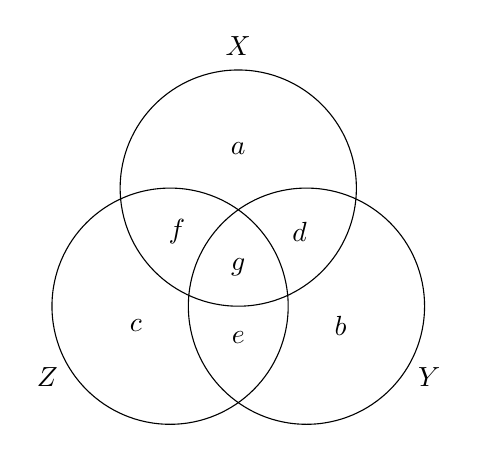
\begin{tikzpicture}
    % circles
    \draw (90:1) circle (1.5);
    \draw (210:1) circle (1.5);
    \draw (330:1) circle (1.5);

    % labels
    \node at (90:2.8) {$X$};
    \node at (330:2.8) {$Y$};
    \node at (210:2.8) {$Z$};
    
    \node at (90:1.5) {$a$};
    \node at (330:1.5) {$b$};
    \node at (210:1.5) {$c$};
    \node at (30:.9) {$d$};
    \node at (270:.9) {$e$};
    \node at (150:.9) {$f$};
    \node at (0:0) {$g$};
  \end{tikzpicture}
  \caption{Partition of $X \cup Y \cup Z$.  The quantities $a,b,c,d,e,f,g$
    represent the cardinalities of each disjoint set as shown.}
  \label{fig:partition}
\end{figure}

The normalised symmetric difference is also a metric on $2^{S}$:
\begin{equation*}
  \delta_{\symdif_n}(X,Y) =
  \begin{cases}
    \displaystyle \frac{|X \symdif Y|}{|X \cup Y|} & \text{if $X \cup Y \neq
      \emptyset$} \\
    0 & \text{otherwise.}
  \end{cases}
\end{equation*}

\begin{proof}
  The proof shown here is from \citep{yianilos91}, with some corrections.
  Again, it is easy to see the function is non-negative, symmetric and that
  $\delta_{\symdif_n}(X,Y)=0$ if and only if $X=Y$ for all $X,Y \in 2^{\dset}$
  so we will show that the triangle inequality holds which is:
  \begin{equation*}
    \frac{|X \symdif Y|}{|X \cup Y|} + \frac{|Y \symdif Z|}{|Y \cup Z|} \geq
    \frac{|X \symdif Z|}{|X \cup Y|}
  \end{equation*}
  or, equivalently:
  \begin{equation}
    \label{eq:tri-inequality}
    1 - \frac{|X \cap Y|}{|X \cup Y|} +
    1 - \frac{|Y \cap Z|}{|Y \cup Z|} \geq
    1 - \frac{|X \cap Z|}{|X \cup Z|}.
  \end{equation}

  We partition $X \cup Y \cup Z$ into disjoint subsets as shown in
  Figure~\ref{fig:partition} and let
  \begin{align*}
    a &= |X \setminus (Y \cup Z)|\\
    b &= |Y \setminus (X \cup Z)|\\
    c &= |Z \setminus (X \cup Y)|\\
    d &= |(X \cap Y) \setminus Z|\\
    e &= |(Y \cap Z) \setminus X|\\
    f &= |(Z \cap X) \setminus Y|\\
    g &= |X \cap Y \cap Z|
  \end{align*}
  and for convenience we let
  \begin{equation*}
    \xi  = |X \cup Y \cup Z|.
  \end{equation*}

  We can now write equation~(\ref{eq:tri-inequality}) as
  \begin{equation*}
    1 - \frac{d+g}{\xi -c} + 1 - \frac{e+g}{\xi -a} \geq 1 - \frac{f+g}{\xi -b}
  \end{equation*}
  which can be rewritten as
  \begin{equation*}
    \frac{d+g}{\xi -c} + \frac{e+g}{\xi -a} \leq \frac{f+g}{\xi -b} + 1.
  \end{equation*}

  Removing $b$ from the denominators on the LHS can only make the LHS
  greater, so it is sufficient to show that
  \begin{equation*}
    \frac{d+g}{\xi -b-c} + \frac{e+g}{\xi -a-b} \leq \frac{f+g}{\xi -b} + 1.
  \end{equation*}

  Now if we replace $1$ with $\frac{\xi -a-b-c}{\xi -a-b-c}$ on the RHS and add
  the fractions on the LHS we get
  \begin{multline*}
    \frac{(\xi -a-b)(d+g)+(\xi -b-c)(e+g)}{(\xi -b-c)(\xi -a-b)}\\
    \leq \frac{(\xi -a-b-c)(\xi -b)+(\xi -a-b-c)(f+g)}{(\xi -b)(\xi -a-b-c)}
  \end{multline*}
  which when we expand the denominators becomes
  \begin{multline*}
    \frac{(\xi -a-b)(d+g)+(\xi -b-c)(e+g)}{\xi ^2-\xi a-2\xi b-\xi c+ab+bc+b^2+ac}\\
    \leq \frac{(\xi -a-b-c)(\xi -b)+(\xi -a-b-c)(f+g)}{\xi ^2-\xi a-2\xi b-\xi c+ab+bc+b^2}.
  \end{multline*}
  Notice that the denominator on the LHS is equal to the denominator on the
  RHS with the addition of $ac$ so it cannot be less.  It is therefore
  sufficient to show that
  \begin{multline*}
    (\xi -a-b)(d+g)+(\xi -b-c)(e+g)\\
    \leq (\xi -a-b-c)(\xi -b)+(\xi -a-b-c)(f+g).
  \end{multline*}

  Starting with the LHS we have
  \begin{align*}
    &(\xi -a-b)(d+g)+(\xi -c-b)(e+g)\\
    &= (\xi -a-b-c)(d+g)+c(d+g)+(\xi -a-b-c)(e+g)+a(e+g)\\
    &\leq (\xi -a-b-c)(d+g)+c(\xi -a-b-c)\\
    &\qquad\qquad+(\xi -a-b-c)(e+g)+a(\xi -a-b-c)\\
    &= c(\xi -a-b-c)+(\xi -a-b-c)(d+e+g)\\
    &\qquad\qquad+g(\xi -a-b-c)+a(\xi -a-b-c)\\
    &\leq c(\xi -a-b-c)+(\xi -a-b-c)^2+g(\xi -a-b-c)+a(\xi -a-b-c)\\
    &= (\xi -a-b-c)(\xi -b)+g(\xi -a-b-c)\\
    &\leq (\xi -a-b-c)(\xi -b) + (f+g)(\xi -a-b-c).
  \end{align*}
\end{proof}

\begin{figure}
  \centering
  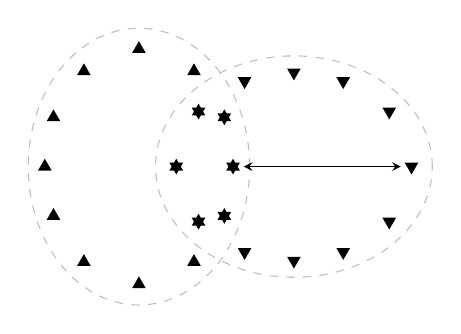
\begin{tikzpicture}[
    node1/.style={dot,regular polygon,regular polygon sides=3,
      minimum size=2mm,fill=black},
    node2/.style={dot,regular polygon,regular polygon sides=3,
      minimum size=2mm,fill=black,rotate=180}
    ]

    \draw [dashed,faint] (-2.8em,0) ellipse (4em and 5em);
    \draw [dashed,faint] (2.8em,0) ellipse (5em and 4em);

    % set 1 primary markers
    \begin{scope}[xshift=-2.8em,scale=0.85]
      \foreach \theta in {0,30,...,330} {
        \pgfmathparse{(4*5)/sqrt((5*cos(\theta))^2+(4*sin(\theta))^2)}
        \node [node1] (1set\theta) at (\theta:\pgfmathresult em) {};
      }
    \end{scope}
    % set 2 markers
    \begin{scope}[xshift=-2.8em,scale=0.85]
      \foreach \theta in {0,30,330} {
        \pgfmathparse{(4*5)/sqrt((5*cos(\theta))^2+(4*sin(\theta))^2)}
        \node [node2] at (\theta:\pgfmathresult em) {};
      }
    \end{scope}

    % set 2 primary markers
    \begin{scope}[xshift=2.8em,scale=0.85]
      \foreach \theta in {0,30,...,330} {
        \pgfmathparse{(5*4)/sqrt((4*cos(\theta))^2+(5*sin(\theta))^2)}
        \node [node2] (2set\theta) at (\theta:\pgfmathresult em) {};
      }
    \end{scope}
    % set 1 markers
    \begin{scope}[xshift=2.8em,scale=0.85]
      \foreach \theta in {150,180,210} {
        \pgfmathparse{(5*4)/sqrt((4*cos(\theta))^2+(5*sin(\theta))^2)}
        \node [node1] at (\theta:\pgfmathresult em) {};
      }
    \end{scope}

    \draw [symdist] (2set0) -- (1set0);
  \end{tikzpicture}
  \caption{The Haussdorf distance between two subsets of a metric space can be
    described informally as the greatest distance one must travel if starting
    from a point in one set and travelling to the closest point in the other
    set.  This distance is marked in the diagram.}
  \label{fig:haussdorf}
\end{figure}

If the sets are nonempty subsets of a metric space, $(M,d)$, then the
underlying metric space can be used to define metrics on the sets.  The
Haussdorf metric is a metric on $2^{M}$ \citep{braun2003geometry}:
\begin{equation*}
  \delta_{H}(X,Y) = \max\left(\max_{x \in X} \min_{y \in Y} d(x,y),
                             \max_{y \in Y} \min_{x \in X} d(x,y)\right).
\end{equation*}
This distance is illustrated in Figure~\ref{fig:haussdorf}.  In
Chapter~\ref{cha:assignment-metric} we present another metric which can be
used for this purpose.

As an aside, it should be noted that linkage functions, which are used in
hierarchical clustering, the topic of Section~\ref{sec:hierarchies}, are not
generally metrics.  The \textit{single-linkage distance}:
\begin{equation*}
  \delta(X,Y) = \min_{x \in X, y \in Y} d(x,y)
\end{equation*}
is a simple and intuitive distance between sets, but is not a metric since
distinct sets can have a distance of zero.  \textit{Complete-linkage} and
\textit{average-linkage} are, in fact, not even distances.  These measures
will be discussed in Section~\ref{sec:hierarchies}.

\subsection{Other metrics}
\label{sec:other-metrics}

Many other metrics exist including the Hellinger distance and Jensen-Shannon
divergence squared \citep{endres03metric} for probability distributions.
There exist generalised Mahalanobis distances for mixed data
\citep{leon2005generalized}.  In Section~\ref{sec:comparing-partitions} we
look at metrics (and general dissimilarities) on partitions and in
Chapter~\ref{cha:assignment-metric} we introduce our own metric.

It is also possible in some cases to transform a general dissimilarity into a
metric, for example see \citet[chap. 2.5]{everitt80}.

\subsection{Multiset datasets}
\label{sec:multiset-datasets}

It is tempting to think of a dataset and a metric defined on its elements as a
metric space, but this is not necessarily correct.  The reason is that,
contrary to the name, a dataset is not usually a set but a multiset.  Consider
a dataset consisting of only the heights of some population of humans.
Depending on the precision of the measurements taken, it would generally be
expected that multiple subjects share the same height.  In order to have these
observations in a set, some unique integer---an experiment number, say---would
need to be attached to each observation.  But then the metric condition that
$d(x,y)=0$ only if $x=y$ would be violated---in fact we would have only a
\textit{pseudometric}.  We can get a proper metric if we define an equivalence
relation $x \sim y$ if $d(x,y)=0$.  Then $(\dset/\sim,d)$ is a metric space.

Most of the time we do not need to worry about this.  From now on a dataset,
$\dset$, will implicitly mean $\dset/\sim$ as defined above unless stated
otherwise.  Occasionally. though, it will be useful or necessary to consider
the multiset $(\dset,\mu_{\dset})$ where $\dset$ is the underlying set, and
$\mu_{\dset} \colon \dset \to \mathbb{N}_1$---a map from $\dset$ to the
(nonzero) natural numbers---is called the membership function and tells us how
many times an element appears in the multiset.

A further generalisation is then possible: we can relax the definition of the
membership function to $\mu_{\dset} \colon \dset \to \mathbb{R}_1$---a map
from $\dset$ to the positive real numbers.  The dataset is then a fuzzy
multiset.  Such datasets have been used in document clustering applications,
for example in \citep{miyamoto2003information}, where objects can appear
multiple times with a certain probability attached.  If the membership
function if $\mu_{\dset} \colon \dset \to \mathbb{R}_1 \cap [0,1]$ then
$(\dset,\mu_{\dset})$ is called a fuzzy set
\citep{zadeh1965fuzzy,gottwald2010fuzzy}.

\section{Partitions}
\label{sec:partitions}

In this section we look at the properties of partitions of sets, how we can
compare partitions and how we can find partitions.

\subsection{The space of partitions}
\label{sec:space-partitions}

A $k$-partition, $\clus = \{C_1,C_2,\dotsc,C_k\}$, of an $n$ element set,
$\dset$, is a set of $k \in \{1,2,\dotsc,n\}$ non-empty, pairwise disjoint
subsets such that $C_1 \cup C_2 \cup \dotsb \cup C_k = \dset$.  Following
common practice, we will refer to the elements of $\clus$ as
\textit{clusters}.

\begin{figure}
  \centering
  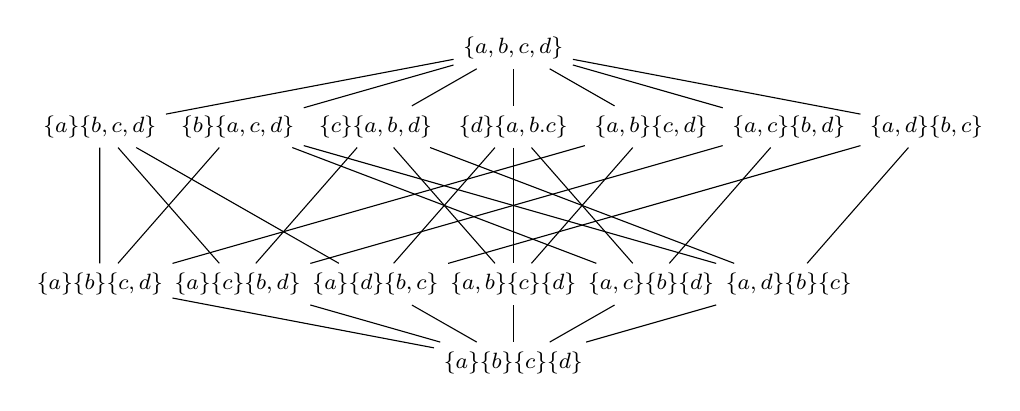
\begin{tikzpicture}[
    xscale=1.75, font=\footnotesize]

    % vertices
    
    \node (0) at (0,0) {$\{a,b,c,d\}$};

    \node (10) at (-3,-1) {$\{a\}\{b,c,d\}$};
    \node (11) at (-2,-1) {$\{b\}\{a,c,d\}$};
    \node (12) at (-1,-1) {$\{c\}\{a,b,d\}$};
    \node (13) at (0,-1) {$\{d\}\{a,b.c\}$};
    \node (14) at (1,-1) {$\{a,b\}\{c,d\}$};
    \node (15) at (2,-1) {$\{a,c\}\{b,d\}$};
    \node (16) at (3,-1) {$\{a,d\}\{b,c\}$};

    \node (20) at (-3,-3) {$\{a\}\{b\}\{c,d\}$};
    \node (21) at (-2,-3) {$\{a\}\{c\}\{b,d\}$};
    \node (22) at (-1,-3) {$\{a\}\{d\}\{b,c\}$};
    \node (23) at (0,-3) {$\{a,b\}\{c\}\{d\}$};
    \node (24) at (1,-3) {$\{a,c\}\{b\}\{d\}$};
    \node (25) at (2,-3) {$\{a,d\}\{b\}\{c\}$};

    \node (3) at (0,-4) {$\{a\}\{b\}\{c\}\{d\}$};

    % edges

    \draw (0) to (10);
    \draw (0) to (11);
    \draw (0) to (12);
    \draw (0) to (13);
    \draw (0) to (14);
    \draw (0) to (15);
    \draw (0) to (16);

    \draw (10) to (20);
    \draw (10) to (21);
    \draw (10) to (22);
    \draw (11) to (20);
    \draw (11) to (24);
    \draw (11) to (25);
    \draw (12) to (21);
    \draw (12) to (23);
    \draw (12) to (25);
    \draw (13) to (22);
    \draw (13) to (23);
    \draw (13) to (24);
    \draw (14) to (20);
    \draw (14) to (23);
    \draw (15) to (21);
    \draw (15) to (24);
    \draw (16) to (22);
    \draw (16) to (25);

    \draw (20) to (3);
    \draw (21) to (3);
    \draw (22) to (3);
    \draw (23) to (3);
    \draw (24) to (3);
    \draw (25) to (3);
  \end{tikzpicture}
  \caption{The Hasse diagram of the lattice of partitions of a set,
    $\dset=\{a,b,c,d\}$ \citep{meila-2005}.  Each vertex in the graph is a
    partition $\{C_1,\dotsc,C_k\}$ of $\dset$ which we denote by
    $C_1,\dotsc,C_k$ for clarity.}
  \label{fig:lattice}
\end{figure}

The set, $\parts_{\dset}$, of all partitions of $\dset$ forms a lattice called
the \textit{lattice of partitions}.  A lattice can be represented as a graph
called a \textit{Hasse diagram} with vertex set $\parts_{\dset}$ and edge set
consisting of edges $(\clus_1,\clus_2) \in \parts_{\dset}
\times \parts_{\dset}$ such that a cluster in $\clus_1$ is the union of two
clusters in $\clus_2$.  In general, we call $\clus_2$ a \textit{refinement} of
$\clus_1$.

The Hasse diagram of a four element set is shown in Figure~\ref{fig:lattice}.
The partition at the top is the partition that is not a refinement of any
partition ($k=1$).  The partition at the bottom is the partition that is a
refinement of every other partition ($k=n$).

As this example suggests, a set can support a large number of possible
partitions.  We can count the number of possible partitions of an $n$ element
set using the \textit{Bell number}, $B_n$
\citep{bell1934exponential,stanley2000enumerative}, which is defined by $B_0 =
1$ and the recursive formula:
\begin{equation*}
  B_n = \sum_{l=0}^{n-1} B_l \binom{n-1}{l} \qquad \text{for $n \geq 1$},
\end{equation*}
and, alternatively, Dobinski's formula \citep{dobinski1877summation}:
\begin{equation*}
  B_n = \frac{1}{e} \sum_{l=0}^{\infty} \frac{l^n}{l!} \qquad \text{for $n
    \geq 0$}.
\end{equation*}
We illustrate the growth of the Bell numbers in Table~\ref{tab:bell-number}.

\begin{table}
  \centering
  \begin{tabular}{rr}
    \toprule
    $n$ & $B_n$ \\
    \midrule
    5 & 52 \\
    10 & 115,975 \\
    15 & 1,382,958,545 \\
    20 & $5.17 \times 10^{13}$ \\
    25 & $4.64 \times 10^{18}$ \\
    \bottomrule
  \end{tabular}
  \caption{The value of the Bell number, $B_n$, for some selected values of
    $n$.}
  \label{tab:bell-number}
\end{table}

\subsubsection{Fuzzy partitions}
\label{sec:fuzzy-partitions}

Partitions can be generalised to fuzzy partitions by letting the clusters be
fuzzy sets.  Fuzzy sets are collections of objects where each member of a
collection has a grade of membership associated to it \citep{zadeh1965fuzzy}.
Sets are a special case where the grades of membership are binary---objects
are either members of a set or they are not.  Fuzzy sets and partitions have
many applications including classification of data in the natural sciences
where membership is not precisely defined.

A fuzzy set is an ordered pair, $(C,\mu_{C})$, consisting of an underlying
set, $C$, and a membership function $\mu_{C} \colon C \to (0,1]$.  Note that
in our definition, all members of the underlying set are members to some
extent of the fuzzy set since the grade of membership cannot be zero.

A \textit{$k$-fuzzy-partition} of an $n$ element set, $\dset$, is a set of $k
\in \{1,2,\dotsc,n\}$ fuzzy sets,
$\{(C_1,\mu_1),(C_2,\mu_2),\dotsc,(C_k,\mu_k)\}$, where $C_1 \cup C_2 \cup
\dotsb \cup C_k = \dset$, $C_i \neq \emptyset$ for all $1 \leq i \leq k$ and
$\sum_{i=1}^{k} \mu_i(x) = 1$ for all $x \in \dset$.  For convenience we
denote each membership function $\mu_{C_i}$ as simply $\mu_i$.  The underlying
sets of the clusters are not necessarily pairwise disjoint, so elements can
belong to more than one cluster.

\subsection{Comparing partitions}
\label{sec:comparing-partitions}

An attractive way to find partitions of a set is by means of a partitional
clustering method.  Many methods exist---we will review some in
Section~\ref{sec:part-clust-algor}---and, depending on their respective
approach to the problem, they all tend to produce different partitions.  To
further complicate matters, some methods are non-deterministic and produce
different partitions each time they are used.

For the purposes of comparing and assessing clustering methods it is therefore
useful to be able to compare partitions.  Many measures have been devised for
this purpose, including similarity measures and dissimilarity measures, of
which some are metrics.  Existing methods fall into four main categories; for
two partitions, $\clus_1$ and $\clus_2$, of a set $\dset$, these are:
\begin{description}
\item[Pair counting] which measures the agreement and disagreement between
  $\clus_1$ and $\clus_2$ by means of counting pairs of element in the set,
\item[Set matching] which ``matches'' clusters in $\clus_1$ with clusters in
  $\clus_2$ and measures the similarity between matched sets,
\item[Information theoretic] which uses information theory to measure the
  information and mutual information contained in $\clus_1$ and $\clus_2$,
\item[Density profile] which takes into account the values of the data when
  computing the measure.
\end{description}

We will review measures belonging to the first three categories in this
section.  The fourth category consists of a single measure called ADCO which
we will analyse in Chapter~\ref{cha:assignment-metric}.

To be able to describe the measures in detail, we need to introduce some more
terminology.  As before, let $\dset = \{x_1,x_2,\dotsc,x_n\}$ be a set of $n
\geq 2$ elements and $\clus_1 = \{C_{11},C_{12},\dotsc,C_{1k}\}$ and $\clus_2
= \{C_{21},C_{22},\dotsc,C_{2k'}\}$ be two partitions of $\dset$ with $k$ and
$k'$ clusters respectively.

We denote, for some $x \in \dset$, and a partition, $\clus$, of $\dset$, the
cluster in $\clus$ that contains $x$ by $\clus(x)$.

The \textit{confusion matrix} of two partitions, $\clus_1$ and $\clus_2$, is
the $k \times k'$ matrix $[n_{ij}]$ where $n_{ij} = |C_{i1} \cap C_{2j}|$.
The confusion matrix is used for the calculation of both pair counting and set
matching measures.

To illustrate these definitions and the comparison measures we will use two
example partitions, $\clus^*_1$ and $\clus^*_2$, on a set, $\dset^* =
\{1,2,\dotsc,9\}$, throughout this section:
\begin{align*}
  \clus^*_1 &= \{C^*_{11},C^*_{12},C^*_{13}\}, \\
  \clus^*_2 &= \{C^*_{21},C^*_{22},C^*_{23},C^*_{24}\}
\end{align*}
where
\begin{align*}
  C^*_{11}&=\{1,2,3\},C^*_{12}=\{4,5,6\},C^*_{13}\{7,8,9\}, \\
  C^*_{21}&=\{1,4\},C^*_{22}=\{2,3,6\},C^*_{23}=\{5,8\},C^*_{24}\{7,9\}.
\end{align*}
Then, for example, we have $\clus^*_1(3) = C^*_{11}$.  The confusion matrix
associated with $\clus^*_1$ and $\clus^*_2$ is:
\begin{equation*}
  [n_{ij}]^*=\left[
  \begin{matrix}
    1 & 2 & 0 & 0 \\
    1 & 1 & 1 & 0 \\
    0 & 0 & 1 & 2
  \end{matrix}
  \right]
\end{equation*}

\subsubsection{Pair counting}
\label{sec:pair-counting}

There are $\binom{n}{2}$ distinct pairs of elements in $\dset$.  For each
distinct pair $(a,b) \in \dset \times \dset$ one of the following is true:
\begin{itemize}
\item $a,b$ are in the same cluster in $\clus_1$ and the same cluster in
  $\clus_2$,
\item $a,b$ are in different clusters in $\clus_1$ and different clusters in
  $\clus_2$,
\item $a,b$ are in the same cluster in $\clus_1$ but in different clusters in
  $\clus_2$,
\item $a,b$ are in different clusters in $\clus_1$ but in the same cluster in
  $\clus_2$.
\end{itemize}

Counting the number of element in each category gives us four counts which are
defined formally as:
\begin{align*}
  N_{11} &= |\{(a,b) \in \dset \times \dset \colon
              \clus_1(a)=\clus_1(b) \text{ and } \clus_2(a)=\clus_2(b)
            \}|, \\
  N_{00} &= |\{(a,b) \in \dset \times \dset \colon
              \clus_1(a)\neq\clus_1(b) \text{ and } \clus_2(a)\neq\clus_2(b)
            \}|, \\
  N_{10} &= |\{(a,b) \in \dset \times \dset \colon
              \clus_1(a)=\clus_1(b) \text{ and } \clus_2(a)\neq\clus_2(b)
            \}|, \\
  N_{01} &= |\{(a,b) \in \dset \times \dset \colon
              \clus_1(a)\neq\clus_1(b) \text{ and } \clus_2(a)=\clus_2(b)
            \}|.
\end{align*}

The size of $N_{11}$ and $N_{00}$ are considered to be measurements of the
agreement between the $\clus_1$ and $\clus_2$, while $N_{10}$ and $N_{01}$ are
considered measurements of the disagreement between them.  The measures based
on pair counting can all be expressed in terms of these four counts.  Clearly
$N_{11}+N_{00}+N_{10}+N_{01} = \binom{n}{2}$ is always satisfied.  The counts
can all be obtained from the confusion matrix using the following formul\ae
\citep{hubert-arabie-1985}:
\begin{align*}
  N_{11} &= \frac{1}{2} \sum_{i=1}^{k} \sum_{j=1}^{k'} n_{ij}(n_{ij}-1),\\
  N_{00} &= \frac{1}{2} \left(n^2 + \sum_{i=1}^{k} \sum_{j=1}^{k'} n_{ij}^2
                             - \sum_{i=1}^{k}
                                \left(\sum_{j=1}^{k'} n_{ij} \right)^2
                             - \sum_{j=1}^{k'}
                                \left(\sum_{i=1}^{k} n_{ij} \right)^2
                       \right),\\
  N_{10} &= \frac{1}{2} \left(\sum_{i=1}^{k}
                              \left(\sum_{j=1}^{k'} n_{ij} \right)^2
                             - \sum_{i=1}^{k} \sum_{j=1}^{k'} n_{ij}^2
                       \right),\\
  N_{01} &= \frac{1}{2} \left(\sum_{j=1}^{k'}
                              \left(\sum_{i=1}^{k} n_{ij} \right)^2
                             - \sum_{i=1}^{k} \sum_{j=1}^{k'} n_{ij}^2
                       \right).
\end{align*}

One of the simplest pair counting measures between two partitions, $\clus_1$
and $\clus_2$, is the widely-used \textit{Rand index}, $\partcompare{R}$,
introduced in \citep{rand-1971} and defined as:
\begin{equation*}
\partcompare{R} = \frac{(N_{11}+N_{00})}{\binom{n}{2}}.
\end{equation*}
The Rand index is a similarity measure with a lower bound of 0 and an upper
bound of 1.  \citet{hubert-arabie-1985} use the following variation:
\[\partcompare{HA} = (N_{11}+N_{00}-N_{10}-N_{01})/\binom{n}{2}\].

\citet{wallace-1983} introduced two asymmetric measures,
$\mathcal{W}_{I}(\clus_1,\clus_2)$ and $\mathcal{W}_{II}(\clus_1,\clus_2)$
defined as:
\begin{equation*}
  \mathcal{W}_{I}(\clus_1,\clus_2) =
  \frac{N_{11}}{\sum_{i=1}^{k} |C_{i1}|(|C_{1i}|-1)/2},
\end{equation*}
and
\begin{equation*}
  \mathcal{W}_{II}(\clus_1,\clus_2) =
  \frac{N_{11}}{\sum_{j=1}^{k'} |C_{2j}|(|C_{2j}|-1)/2}.
\end{equation*}
$\mathcal{W}_{I}$ and $\mathcal{W}_{II}$ represent the probabilities that, for
a pair of elements $(a,b) \in \dset \times \dset$ with
$\clus_1(a)=\clus_1(b)$, we also have $\clus_2(a)=\clus_2(b)$, and vice versa.
A symmetric similarity measure can be obtained from Wallace's measures by
taking their geometric mean:
\begin{equation*}
  \partcompare{F} = \sqrt{\mathcal{W}_{I}(\clus_1,\clus_2)
                          \mathcal{W}_{II}(\clus_1,\clus_2)}.
\end{equation*}
This measure was also introduced independently by Fowlkes and Mallows in
\citep{fowlkes-mallows-1983}.

The Jaccard coefficient, $\partcompare{J}$, is another widely-used similarity
measure and is defined, for $\clus_1$ and $\clus_2$, as:
\begin{equation*}
  \partcompare{J} = \frac{N_{11}}{N_{10}+N_{01}+N_{11}}.
\end{equation*}

It should be noted that all measures reviewed so far are similarity measures.
The \textit{Mirkin metric}, $\partcompare{M}$, for measuring dissimilarity
between two partitions, $\clus_1$ and $\clus_2$, was originally introduced in
\citep{mirkin1996mathematical} and is defined as
\begin{equation*}
  \partcompare{M} = \sum_{i=1}^{k} |C_{1i}|^2 +
                    \sum_{j=1}^{k'} |C_{1j}|^2 +
                    2\sum_{i=1}^{k}\sum_{j=1}^{k'} n_{ij}^2,
\end{equation*}
where $n_{ij}$ again denotes the confusion matrix associated with $\clus_1$
and $\clus_2$.  As it turns out, $\partcompare{M}=2(N_{10}+N_{01})$.  A
closely related measure, $\partcompare{AB}=(N_{10}+N_{01})/\binom{n}{2}$, is
also a metric and was used by \citet{mirkin1970measurement} and
\citet{arabie1973multidimensional}.

\begin{table}
  \centering
  \begin{tabular}{lr}
    \toprule
    Name & Measure \\
    \midrule
    Rand index          & $\partcomparest{R} \approx 0.694$ \\
    Wallace measures    & $\mathcal{W}_{I}(\clus^*_1,\clus^*_2) \approx 0.222$ \\
                        & $\mathcal{W}_{II}(\clus^*_1,\clus^*_2) \approx 0.333$ \\
    Fowlkes \& Mallows  & $\partcomparest{F} \approx 0.272$ \\
    Jaccard coefficient & $\partcomparest{J} \approx 0.154$ \\
    Merkin metric       & $\partcomparest{M} = 22.00$ \\
    \bottomrule
  \end{tabular}
  \caption{Various pair counting based measures applied to the partitions
    $\clus_1$ and $\clus_2$.}
  \label{tab:pair-counting-comparison}
\end{table}

The four counts for our example partitions, $\clus^*_1$ and $\clus^*_2$, are:
\begin{equation*}
  N_{11} = 2,\quad
  N_{00} = 23,\quad
  N_{10} = 7,\quad
  N_{01} = 4.
\end{equation*}
The values of the reviewed pair counting measures when applied to $\clus^*_1$
and $\clus^*_2$ are given in Table~\ref{tab:pair-counting-comparison}.

\subsubsection{Set matching}
\label{sec:set-matching}

Set matching measures are based on comparisons between matched pairs of
clusters.  Each pair consists of a cluster from each partition that is being
compared.  All existing measures use the cardinality of the intersection
between two clusters as a similarity measure for comparison.  This is given by
the confusion matrix.  The differences between the measures are essentially
due to the way that they find the matched pairs for comparison.

As before, let $\clus_1 = \{C_{11},\dotsc,C_{1k}\}$ and $\clus_2 =
\{C_{21},\dotsc,C_{1k'}\}$, where $k,k' \geq 1$, be two partitions of an $n$
element set, $\dset$.  Assume, without loss of generality, that $k' \geq k$.
Then, a matching between $\clus_1$ and $\clus_2$ is a function $\sigma \colon
\{1,\dotsc,k\} \to \{1,\dotsc,k'\}$.  A possible matching for a pair of
partitions is shown in figure~\ref{fig:matching}.

\begin{figure}
  \Centering
  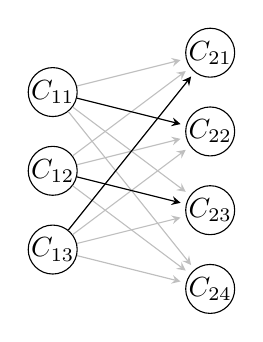
\begin{tikzpicture}[
    % >=stealth,
    % clus/.style={circle,draw=black,inner sep=0,minimum size=5mm},
    % dist/.style={->,shorten >=2pt},
    % faint/.style={dist,gray!50},
    nonmatch/.style={dist,faint},
    match/.style={dist,black}
    ]

    \node [clus] (c11) at (0,1) {$C_{11}$};
    \node [clus] (c12) at (0,0) {$C_{12}$};
    \node [clus] (c13) at (0,-1) {$C_{13}$};

    \node [clus] (c21) at (2,1.5) {$C_{21}$};
    \node [clus] (c22) at (2,.5) {$C_{22}$};
    \node [clus] (c23) at (2,-.5) {$C_{23}$};
    \node [clus] (c24) at (2,-1.5) {$C_{24}$};

    % join them all
    \foreach \x in {1,2,3} {
      \foreach \y in {1,2,3,4} {
        \draw [nonmatch] (c1\x) to (c2\y);
      }
    }

    % matches
    \draw [match] (c11) to (c22);
    \draw [match] (c12) to (c23);
    \draw [match] (c13) to (c21);
  \end{tikzpicture}
  \caption{One possible matching between partitions $\{C_{11},\dotsc,C_{13}\}$
    and $\{C_{21},\dotsc,C_{24}\}$.  In this case, the matching is an
    injection.}
  \label{fig:matching}
\end{figure}

\citet{meila-2001} introduced a set matching measure for the similarity
between two partitions.  It finds a matching using the following heuristic:
let $[n_{ij}]$ be the $k \times k'$ confusion matrix associated with $\clus_1$
and $\clus_2$.  Compute $n_{ab} = \argmax \{n_{ij} \colon 1 \leq i \leq k, 1
\leq j \leq k'\}$ and put $\sigma(a) \gets b$.  Repeat the process for the
$(k-1) \times (k'-1)$ submatrix obtained by deleting row $a$ and column $b$,
and so on until $k$ matches have been made.  This process give us an injection
for $\sigma$ and the measure is then defined as:
\begin{equation*}
  \partcompare{H} = \frac{1}{n} \sum_{i=1}^{k} n_{i \sigma(i)}.
\end{equation*}

A second similarity measure, $\partcompare{L}$, introduced by
\citet{larsen-aone-1999}, simply computes a maximal matching for each cluster:
\begin{equation*}
  \partcompare{L} = \frac{1}{k} \sum_{i=1}^{k} \max_{1 \leq j \leq k'}
                                             \frac{2n_{ij}}{|C_{1i}|+|C_{2j}|}.
\end{equation*}

A dissimilarity measure, $\partcompare{V}$, which is a metric, was introduced
by \citet{van-dongen-2000}.  This measure, again, computes maximal matchings
for each cluster:
\begin{equation*}
  \partcompare{V} = 2n - \sum_{i=1}^{k} \max_{1 \leq j \leq k'} n_{ij}
                         \sum_{j=1}^{k'} \max_{1 \leq i \leq k} n_{ij}.
\end{equation*}

A second metric, $\partcompare{CE}$, is due to \citet{meila-2005} and is know
as \textit{classification error}.  Like $\partcompare{H}$, this measure
computes an injection for $\sigma$, but instead of using a heuristic, the
globally optimal injection is found among all possible injections, $S_k$:
\begin{equation*}
  \partcompare{CE} = 1 - \frac{1}{n} \max_{\sigma \in S_k}
                                     \sum_{i=1}^{k} n_{i \sigma(i)}.
\end{equation*}
Note that the injection, $\sigma$, can be found in polynomial time.  Also,
$\partcompare{CE} \leq 1$ for all partitions $\clus_1$ and $\clus_3$ on
$\dset$.

\begin{table}
  \centering
  \begin{tabular}{lr}
    \toprule
    Name & Measure \\
    \midrule
    Meilă \& Heckerman   & $\partcompare{H} \approx 0.556$ \\
    Larsen \& Aone       & $\partcompare{L} \approx 0.622$ \\
    Van Dongen metric    & $\partcompare{V} = 7.000$ \\
    Classification Error & $\partcompare{CE} \approx 0.445$ \\
    
    \bottomrule
  \end{tabular}
  \caption{Various set matching based measures applied to $\clus_1$ and $\clus_2$.}
  \label{tab:set-matching-comparison}
\end{table}

The values of the set matching measures when applied to our example partitions
are given in Table~\ref{tab:set-matching-comparison}.

\citet{meila-2007} and \citet{bae2010comparison} point out that all of these
measures suffer from the so-called ``problem of matching'' which we will now
illustrate.  Given a partition, $\clus$, with $k$ equally sized clusters we
can obtain a second partition, $\clus'$, by moving a fraction, $f$, of the
objects from each cluster, $C_{i}$, to $C_{i+1}$, with the indices taken $\mod
k$.  We can obtain a third partition, $\clus''$, from $\clus$ by taking the
same fraction from each cluster and distributing the objects evenly among all
other clusters.  Our intuition would be that the similarity between $\clus$
and $\clus'$ is not the same as the similarity between $\clus$ and $\clus''$.
However,
\begin{align*}
  \partcomparep{H} = \partcomparepp{H},&\quad
  \partcomparep{L} = \partcomparepp{L},\\
  \partcomparep{V} = \partcomparepp{V},&\quad
  \partcomparep{CE} = \partcomparepp{CE}
\end{align*}
whenever $f < 1/2$.

To give a numerical example, let
\begin{equation*}
  \clus = \{\{1,2,3,4,5\},\{6,7,8,9,10\},\{11,12,13,14,15\}\}
\end{equation*}
and $f = 2/5$.  Our other partitions are therefore
\begin{equation*}
\clus' = \{\{1,2,3,14,15\},\{6,7,8,4,5\},\{11,12,13,9,10\}\}
\end{equation*}
and
\begin{equation*}
\clus'' = \{\{1,2,3,9,14\},\{6,7,8,4,15\},\{11,12,13,5,10\}\}.
\end{equation*}
In this case we have
\begin{align*}
  \partcomparep{H} = \partcomparepp{H} = 3/5,&\quad
  \partcomparep{L} = \partcomparepp{L} = 3/5,\\
  \partcomparep{V} = \partcomparepp{V} = 12,&\quad
  \partcomparep{CE} = \partcomparepp{CE} = 2/5.
\end{align*}

\subsubsection{Information theoretic}
\label{sec:inform-theor}

Two measures which use information theory are \textit{Normalized Mutual
  Information} \citep{fred-jain-2003} and \textit{Variation of Information}
\citep{meila-2007}.  We will look at the latter measure now.

Variation of Information is based on both how much information is contained in
each partition and how much information one partition contains about the other
(their mutual information).

Let $\clus_1 = \{C_{11},\dotsc,C_{1k}\}$, where $k \geq 1$, be partition of an
$n$ element set, $\dset$.  The first quantity is measured by
\begin{equation*}
  H(\clus_1) = -\sum_{i=1}^{k} P_1(i) \log_b P_1(i),
\end{equation*}
where
\begin{equation*}
  P_1(i) = \frac{|C_{i1}|}{k}, \qquad \text{for $i = 1,\dotsc,k$}.
\end{equation*}
Informally, $P_1(i)$, is the probability that an object picked randomly from
$\dset$ is in cluster $C_{1i}$.  This measure is sometimes called the
\textit{entropy}.  The base of the logarithm determines the unit of
information; for example, the bases $b=2,b=e$ and $b=10$ give the information
in so-called \textit{bits}, \textit{nits} and \textit{Hartleys}, respectively
\citep[see][]{kullback68information}.

Now, with $\clus_1$ as above and $\clus_2 = \{C_{21},\dotsc,C_{1k'}\}$, where
$k' \geq 1$, the mutual information, $I(\clus_1,\clus_2)$, between $\clus_1$
and $\clus_2$ is given by:
\begin{equation*}
  I(\clus_1,\clus_2) = \sum_{i=1}^{k} \sum_{i=1}^{k'}
                      P_{12}(i,j) \log_b \frac{P_{12}(i,j)}{P_1(i)P_2(j)},
\end{equation*}
where
\begin{equation*}
  P_{12}(i,j) = \frac{|C_{1i} \cap C_{2j}|}{n}, \qquad \text{for $i =
    1,\dotsc,k,j = 1,\dotsc,k'$}.
\end{equation*}
Informally, $P_{12}(i,j)$ is the probability that an object picked randomly
from $\dset$ is in both $C_{1i}$ and $C_{2j}$.

The Variation of Information, $\partcompare{VI}$, between $\clus_1$ and
$\clus_2$ is then defined as:
\begin{equation*}
  \partcompare{VI} = H(\clus_1) + H(\clus_2) - 2I(\clus_1,\clus_2).
\end{equation*}

As it turns out, $\Delta_{\mathcal{VI}}$ is a metric on $\parts_{\dset}$, for
any set $n$ element $\dset$, and has some nice properties.  These include that
it is $n$-invariant, meaning its value depends only on the relative sizes of
the clusters and not on the number of elements in $\dset$.  Further, it is
bounded for all $n$ by
\begin{equation*}
  \partcompare{VI} \leq \log_b n.
\end{equation*}
Finally, if $\max(k,k') \leq k^*$ where $k^* \leq \sqrt{n}$ then
\begin{equation*}
  \partcompare{VI} \leq 2 \log_b k^*
\end{equation*}
holds.

\begin{table}
  \centering
  \begin{tabular}{lr}
    \toprule
    Name & Measure \\
    \midrule
    Information & $H(\clus_1) \approx 1.585$ \\
                & $H(\clus_2) \approx 1.975$ \\
    Mutual information & $I(\clus_1,\clus_2) \approx 0.834$ \\
    Variation of Information & $\partcompare{VI} \approx 1.891$
    \\
    \bottomrule
  \end{tabular}
  \caption{Variation of Information and its components applied to our example
    partitions  $\clus^*_1$ and $\clus^*_2$ using base 2 for the logarithms.}
  \label{tab:vi-comparison}
\end{table}

The values of Variation of Information and its components applied to our
example partitions, $\clus^*_1$ and $\clus^*_2$, are given in
Table~\ref{tab:vi-comparison}.
\\\\
\noindent The final type of measure, density profile based, takes into
account the values of the data contained within the set, $\dset$.  This is
unlike any of the measures reviewed in this section, which are all, in one way
or another, based only on the relative sizes of the clusters.  We will discuss
this type of measure in Chapter~\ref{cha:assignment-metric}.

\section{Partional clustering}
\label{sec:part-clust-algor}

The problem of finding meaningful partitions of a dataset is called
partitional clustering.  Broadly speaking, the applications of partitional
clustering fall into two categories: \textit{data reduction} and
\textit{object classification}.

Data reduction may be necessary when a dataset is large and it is deemed that
only an essence of the data is wanted for a particular application.  For
example, if geographical data is to be displayed on a map then a large dataset
may not be desirable due to the visual clutter it would create.  Clustering
can be used to reduce the dataset into a more visually appealing and usable
subset.

Object classification is concerned with grouping data into a number of
classes.  For example, given a dataset obtained by market research one may
wish to find different classes of consumers in order to observe their habits
and predict future behaviour.  A further example is document clustering is an
important area concerned with clustering on datasets consisting of objects
written in a natural language.  Search engines such as those found on the
World Wide Web use document clustering to suggest ``similar'' documents to the
one the user is currently interested in, amongst other things
\citep{steinbach2000comparison}.

\subsection{Criteria}
\label{sec:criteria}

Informally, a good partition of a dataset is one where the clusters are
homogeneous---meaning objects belonging to the same cluster are similar---and
well-separated---meaning objects belonging to different clusters are
dissimilar.

The task of judging a particular partition of a set based on these informal
standards is often a highly subjective one but, nevertheless, many objective
criteria have been devised for the purposes of automatic clustering.  The aim
of a partitional clustering algorithm is to find a globally optimal solution,
that is a partition which has maximum homogeneity or separation or both,
according to a particular criterion.

\subsubsection{Dissimilairty based criteria}
\label{sec:diss-based-crit}

Let $\dset$ be a nonempty, finite set, $d \colon \dset \times \dset \to
\mathbb{R}^{\geq 0}$ be a dissimilarity on $\dset$ and $C \in \dset$ be some
cluster.  The most general criteria for homogeneity and separation are defined
only using dissimilarities.
\\\\
\noindent Criteria that measure the homogeneity of $C$ include the
\textit{diameter} of $C$, which is defined as the maximum dissimilarity
between two members of the cluster:
\begin{equation*}
  \max_{x,y \in C} d(x,y),
\end{equation*}
the \textit{radius} of $C$, which is defined as the minimum of the maximum
dissimilarities between each member and another member of the cluster:
\begin{equation*}
  \min_{x \in C_i} \max_{y \in C} d(x,y)
\end{equation*}
the \textit{star} of $C$, which is defined as the minimum of the sums of
dissimilarities between each member and every other member of the cluster:
\begin{equation*}
  \min_{c \in C} \sum_{x \in C} d(x,c),
\end{equation*}
and the \textit{clique} of $C$, which is defined as the sum of dissimilarities
between each pair of members of the cluster:
\begin{equation*}
  \sum_{x,y \in C} d(x,y).
\end{equation*}
\\\\
\noindent Criteria that measure the separation of a cluster, $C$, from every
other cluster include the \textit{split} of $C$, which is defined as the
minimum dissimilarity between a member of the cluster and an element outside
of the cluster:
\begin{equation*}
  \min_{x \in C, y \in \dset \setminus C} d(x,y),
\end{equation*}
and the \textit{cut} of $C$, which is defined as the sum of dissimilarities
between all members of the cluster and all elements outside of the cluster:
\begin{equation*}
  \sum_{x \in C} \sum_{y \in \dset \setminus C} d(x,y).
\end{equation*}

Criteria for partitions can then be formed by simply taking the sum over all
clusters in that partition of one of the above criteria.  We call these
criteria \textit{sum-of-diameters}, \textit{sum-of-radii},
\textit{sum-of-stars} and so on.  Alternatively one could simply take the
maximum or minimum value, as appropriate, over the clusters which we would
call \textit{max-diameter}, \textit{max-radius}, \textit{min-cut} and so on.
The aim of the clustering method is then to minimise a criterion for
homogeneity or maximise a criterion for separation.

Some criteria for homogeneity are equivalent to criteria for separation.  Most
notably, minimising sum-of-cliques is equivalent to maximising sum-of-cuts.
Such a criterion is therefore a criterion for both homogeneity and separation.

As it turns out, criteria which only measure one or the other, like min-split
and max-diameter, are often conflicting.  For example, maximising min-split
produces clusters with poor homogeneity, called the \textit{chaining effect},
and minimising max-diameter results in clusters with poor separation, called
the \textit{dissection effect}.  Such criteria are therefore not so useful on
their own, but one could consider a criterion for homogeneity and a criterion
for separation simultaneously.  This is called a bicriterion
\citep{delattre1980bicriterion}.

\subsubsection{Scatter matrix based criteria}
\label{sec:scatter-matrix-based}

If the dataset, $\dset$ is embedded in $m$-dimensional Euclidean space then
the following criteria based on the scatter or dispersion matrix of
\citet{wilks60} are possible.  Suppose $\dset = \{x_1,\dotsc,x_n\} \subset
\mathbb{R}^m$, the \textit{total scatter matrix}, $\mathbf{T}_{\dset}$, is the
$m \times m$ matrix defined as:
\begin{equation*}
  \mathbf{T}_{\dset} = \sum_{i=1}^{n} (x_i - \bar{x})(x_i - \bar{x})^{\mathrm{T}}
\end{equation*}
where $\bar{x}$ is the mean value of $\dset$.

For any partition, $\clus = \{C_1,\dotsc,C_k\}$ of $\dset$, two further
matrices are defined.  The \textit{within-cluster scatter matrix},
$\mathbf{W}_{\clus}$, is defined as:
\begin{equation*}
\mathbf{W}_{\clus} = \sum_{i=1}^{k} \mathbf{T}_{C_i},
\end{equation*}
where $\mathbf{T}_{C_i}$ is the total scatter matrix for cluster $C_i$.  The
\textit{between-cluster scatter matrix}, $\mathbf{B}_{\clus}$, is defined as:
\begin{equation*}
  \mathbf{B}_{\clus} =
  \sum_{i=1}^{k} |C_i| (c_i - \bar{x}) (c_i - \bar{x})^{\mathrm{T}}
\end{equation*}
where $c_i$ is the mean of cluster $C_i$.  These matrices are related by the
equality
\begin{equation*}
  \mathbf{T}_{\dset} = \mathbf{W}_{\clus} + \mathbf{B}_{\clus}.
\end{equation*}

A popular criterion used in clustering algorithms is the minimisation of the
trace of $\mathbf{W_{\clus}}$, denoted $\tr(\mathbf{W_{\clus}})$.  Since
\begin{equation*}
  \tr(\mathbf{T_{\dset}}) = \tr(\mathbf{W_{\clus}}) + \tr(\mathbf{B_{\clus}}),
\end{equation*}
and $\tr(\mathbf{T}_{\dset})$ is a constant, it follow that minimising
$\tr(\mathbf{W_{\clus}})$ is equivalent to maximising
$\tr(\mathbf{B_{\clus}})$.

Intriguingly, $\tr(\mathbf{W}_{\clus})$ is also equivalent to the sum over all
clusters of the sum of Euclidean distances squared between each member of the
cluster and its mean:
\begin{equation}
  \label{eq:tr(W)}
  \tr(\mathbf{W_{\clus}}) = \sum_{i=1}^{k} \sum_{x \in C_i} d_{E}^2(x,c_i),
\end{equation}
where $d_{E}$ is Euclidean distance.  This can be seen easily by examining the
main diagonal of each $\mathbf{W}_{C_i}$, as illustrated here:
\begin{multline*}
  \mathbf{W}_{C_i} = \\
  \sum_{x \in C_i}
  \begin{bmatrix}
    (x_1-c_{i1})^2 & (x_1-c_{i1})(x_2-c_{i2}) & \cdots &
    (x_1-c_{i1})(x_m-c_{im}) \\
    (x_2-c_{i2})(x_1-c_{i1}) & (x_2-c_{i2})^2 & \cdots &
    (x_2-c_{i2})(x_m-c_{im}) \\
    \vdots & \vdots & \ddots & \vdots \\
    (x_m-c_{im})(x_1-c_{i1}) & (x_m-c_{im})(x_2-c_{i2}) & \cdots &
    (x_m-c_{im})^2
  \end{bmatrix}
\end{multline*}
where $x_j$, $c_{ij}$ denotes the $j$th component of $x,c_{i}$ respectively.

Similarly, $\tr(\mathbf{B_{\clus}})$ is equivalent to the sum of Euclidean
distances squares between each cluster centroid and $\bar{x}$, multiplied by
the cluster's cardinality:
\begin{equation}
  \label{eq:tr(B)}
  \tr(\mathbf{B_{\clus}}) = \sum_{i=1}^{k} |C_i| d^2(c_i,x).
\end{equation}

For this reason, $\tr(\mathbf{W}_{\clus})$ is often called ``sum-of-squares'',
but this name is ambiguous since any criterion utilising sums of distances
squared could have this name.  We therefore call the criterion shown in
equation~\eqref{eq:tr(W)} the \textit{centroid-distance}, due to measuring the
distances between elements and centroids, and in general call any criterion
using sums of distances squared a sum-of-squares criterion.  Note that when
centroid-distance is calculated using equation~\eqref{eq:tr(W)}, we can use
any metric in place of $d_{E}$.  If it is calculated using the scatter matrix
then it is implicitly using the Euclidean metric.

The relationship between equations~\eqref{eq:tr(W)} and \eqref{eq:tr(B)} can
also be established by the Huygens-Steiner, or parallel-axis, theorem, which
states that, for any cluster $C \subset \mathbb{R}^m$ with mean $c$ and any
element $s \in \mathbb{R}^m$:
\begin{equation}
  \label{eq:huygens}
  \sum_{x \in C} d_E^2(x,s) = d_E^2(c,s) \dot |C| +
                             \sum_{x \in C} d_E^2(x,c).
\end{equation}

We now use this theorem to establish a relationship between centroid-distance
and sum-of-cliques.  With some $C \subset \mathbb{R}^m$ as before, we
beginning with equation~\eqref{eq:huygens} and assign some $y \in C$ to $s$
and sum over all $y \in C$:
\begin{equation*}
  \sum_{x,y \in C} d_E^2(x,y) = \sum_{y \in C} d_E^2(c,y) \dot |C|
                           + \sum_{x \in C} d_E^2(x,c) \dot |C|
\end{equation*}
and, since $d_E$ is symmetric,
\begin{equation}
  \label{eq:cd-as-equivalence}
  \frac{\displaystyle \sum_{x,y \in C} d_E^2(x,y)}
       {|C|}
  = 2 \sum_{x \in C} d_E^2(x,c).
\end{equation}
So when we use Euclidean distance squared as dissimilarity measure,
centroid-distance for each cluster is equivalent to sum-of-cliques over twice
the cardinality of the cluster.  Since $d_E$ is symmetric this is the same as
only counting pairwise distances once each.

It should also be noted that centroid-distance is, in fact, simply a more
general version of sum-of-stars where the centre need not be a member of the
dataset but is a member of some underlying metric space.

As mentioned, we generally call any criterion involving a metric squared a
sum-of-squares criterion.  We call the numerator of the left-hand side of
equation~\eqref{eq:cd-as-equivalence} \textit{all-squares}, since we sum over
all pairs of distances.  Since sum-of-cliques can generally be used with any
dissimilarity measure we generally count each pair of elements twice, once in
each direction, but for a metric this is obviously redundant.

\citet{friedman1967criteria} suggested two further criteria based on scatter
matrices, these are the minimisation of the determinant of
$\mathbf{W_{\clus}}$ (denoted $\det(\mathbf{W}_{\clus})$), which is sometimes
called \textit{generalised variance}, and the maximisation of
$\tr(\mathbf{B_{\clus}W_{\clus}}^{-1})$.  These criteria tend to produce
clusters of similar shape and size as centroid-distance with the Euclidean
metric \citep{marriott1982optimization}.

A further three criteria based on scatter matrices are discussed in
\citep{marriott1982optimization}, these are
$\prod_{i=1}^{k}\det(\mathbf{W}_i)^{|C_i|}$, which is a generalisation of
$\det(\mathbf{W})$ that allows cluster of different shapes, $n
\log{\det(\mathbf{W})} - 2\sum_{i=1}^{k} |C_i| \log{|C_i|}$ and
$\sum_{i=1}^{k} (|C_i| \log{\det(\mathbf{W}_i)} - 2|C_i|\log{|C_i|})$.
Finally, in \citep{maronna1974} the criterion
$\sum_{i=1}^{k}\det(\mathbf{W}_i)^{\frac{1}{m}}$ was introduced.

All of the criteria based on the scatter matrix tend to produce ellipsoidal
clusters; clusters with other shapes will either not be found or be divided
into small clusters.  Most of them also tend to produce clusters which are
linearly-separable---meaning they are separated by hyperplanes
\citep{marriott1982optimization}.

\subsubsection{Other criteria}
\label{sec:other-criteria}

Some criteria are based on similarities instead of dissimilarities.  One such
example is the \textit{average entity stability} \citep{Rubin67optimal}.  This
criterion considers an object to be stable if it is more attracted to the rest
of the cluster it is currently in than to any other cluster.  Give, a
similarity measure, $s$, the attraction between an object and a cluster is
defined as the average similarity between the object and the members of that
cluster, with respect to $s$.  The clustering criterion is to maximise the
average entity stability over the whole dataset.

Criteria based on information theory are also possible.
\citet{wallace1968information} introduce a clustering program called SNOB
which attempts to optimise one such information measure.

\subsection{Computational complexity}
\label{sec:complexity-issues}

Given the huge space of possible partitions of a dataset, partitional
clustering is intuitively a hard problem.  In fact, as we will see below, it
has been shown that many partitional clustering problems are NP-complete.

We first need to define what we mean by a partitional clustering problem.  A
partition which is a global minimum or maximum solution, whichever is
appropriate, for a particular criterion is called an \textit{optimal
  partition}.  When we speak of a particular criterion we qualify this name
appropriately, so for example a \textit{centroid-distance optimal partition}
is a partition which globally minimised the centroid-distance criterion.

The problem of finding an optimal partition according to any criterion we will
refer to simply as \textit{clustering}, and, again, whenever we speak of a
particular criterion we will qualify the name appropriately, so for example
\textit{centroid-distance clustering} is the problem of finding an optimal
partition with respect to the centroid-distance criterion.

An NP-completeness result refers to a decision problem.  Since clustering
problems are optimisation problems, whenever one is said to be NP-complete we
are actually referring to the decision problem derived from the optimisation
problem.  The general decision problem version of clustering is simply stated:
\begin{problem}{Clustering}
  \instance{A finite, $n$ element set $\dset$, the number of clusters desired
    $k \in \{1,\dotsc,n\}$, a criterion $f \colon \parts_{\dset} \to
    \mathbb{R}^+$ and a bound $B \in \mathbb{R}^+$.}
  \question{Does there exist a partition, $\clus \in \parts_{\dset}$, such
    that $f(\clus) \leq B$?}
\end{problem}
\\\\
\noindent Sum-of-cuts (and therefore sum-of-cliques) is easily seen to be
NP-complete be considering the following classic NP-complete graph problem
\citep{karp72twentyone,gonzalez1982computational}:
\begin{problem}{Max Cut}
  \instance{Graph $G=(V,E)$, weight $w(e) \in \mathbb{Z}^+$ for each $e \in
    E$, positive integer $K$.}
  \question{Is there a partition of $V$ into disjoint sets $V_1$ and $V_2$
    such that the sum of weights of the edges from $E$ that have one endpoint
    in $V_1$ and one endpoint in $V_2$ is at least $K$?}
\end{problem}This is clearly a specific case of sum-of-cuts clustering with
$k=2$ and where a dissimilarity with values in $\{0,1\}$ is used
\citep{garey76simplified}.  An approximate solution to sum-of-cuts is possible
to find in polynomial time, but, interestingly, the approximation problem of
sum-of-cliques remains NP-complete \citep{sahni1976p}.
\\\\
\noindent A number of partitional clustering problems were shown to be in
NP-complete by \citet{brucker1978complexity}.  Among these was max-diameter
clustering, a result which, as it turns out, is directly deducible from the
earlier results of \citet{sahni1976p}.  Max-diameter clustering remains
NP-complete for $k=3$ and when all dissimilarities are in $\{0,1\}$
\citep{gareyjohnson79}.

It was shown in \citet{gonzalez1985clustering} that max-diameter clustering is
NP-complete when the dataset is in 2-dimensional Euclidean space and the
Euclidean metric is used.  It is also shown that for a general dissimilarity
function, even finding an approximate solution to within some known degree of
the optimal is NP-complete.

For a dataset in 1-dimensional Euclidean space the problem is solvable in
polynomial time.  Further, whenever the dissimilarity measure satisfies the
triangle inequality it possible to find an approximate solution efficiently.
\citet{brucker1978complexity} provides an algorithm for finding solutions with
a max-diameter within two times the max-diameter of the optimal solution.

\citet{bern1996approximation} show that, under the Euclidean metric, it is
NP-complete to find approximate solutions with a max-diameter value within
1.969 times the max-diameter of the optimal, and with a max-radius value
within 1.822 times the max-radius of the optimal.
\\\\
\noindent Another result of \citet{brucker1978complexity} is that
sum-of-diameters clustering is NP-complete for $k \geq 3$.
\citet{doddi2000approximation} show that approximate solutions with a
sum-of-diameters within two times the optimal can be found efficiently, but
only when the dissimilarity satisfies the triangle inequality.  If the
triangle inequality is not satisfied then it is shown that, if $P \neq NP$, no
efficient approximation algorithm is possible, even for $k=3$.

In \citet{hansen87sumofdiameters} it is shown that the problem when $k=2$ is
solvable in $O(n^2 \log n)$ time.  It is also shown that minimising any
function of the diameters can be done in $O(n^5)$ time when $k=2$.
\\\\
\noindent In \citet{garey82quant} it is shown that the quantization problem is
NP-complete for $k \geq 2$.  This problem is stated as follows:
\begin{quote}
  A source produces one sample of a random variable $X$ with equiprobable
  values in $\{1,2,\dotsc,n\}$.  The encoder (quantizer) maps $X$ into a
  variable $Y$ with values in $\{1,2,\dotsc,k\}$. The decoder maps $Y$ into a
  decision variable $Z$ with values in $\{1,2,\dotsc,m\}$. If $X = i$ and $Z =
  j$ the resulting distortion is $d_{ij}$.  All entries in the $n \times m$
  matrix $[d_{ij}]$ are zeros or ones. The goal is to find an encoder
  function, $f \colon X \to Y$, and a decoder function, $g \colon Y \to Z$,
  such that the average distortion
  \begin{equation*}
    \frac{1}{n} \sum_{i=1}^{n} d_{ig(f(i))}
  \end{equation*}
  is as small as possible.
\end{quote}
It it easy to see that this problem is equivalent to a specific case of
sum-of-stars clustering where a dissimilarity with values in $\{0,1\}$ is
used.
\\\\
\noindent The above complexity results, especially the last one for
sum-of-stars, has led many authors to believe that centroid-distance
clustering in Euclidean space is also NP-complete.  In fact this was proved
only relatively recently.  It is in fact NP-complete even when $k=2$
\citep{aloise09exact} and for general $k$ in 2-dimensional Euclidean space
\citep{mahajan09}.  If both $k$ and the number of dimensions, $m$, are fixed,
then the problem is exactly solvable in $O(n^{mk+1} \log n)$ time
\citep{inaba94weightedvoronoi}.

We conclude with remarking that not all clustering problems are hard.  One
example is min-split clustering for which a polynomial time algorithm exists.
In particular, the problem is solved with the single-link hierarchical
clustering algorithm of \citet{johnson67hierarchical}.  The runtime of this
algorithm is $O(n^2)$ \citep{delattre1980bicriterion}.  However, this
criterion does suffer from the previously mentioned chaining effect and for
this reason it is often paired with a criterion for homogeneity in a
bicriterion, effectively making it a hard problem again
\citep{delattre1980bicriterion}.

\subsection{Methods}
\label{sec:methods}

The consequence of the complexity issues discussed in the previous section are
that heuristic methods for approximating optimal solutions are very
prevalent.  There are only a small handful of algorithms which are either
guaranteed to find a globally optimal solution or guaranteed to find a
solution within a known degree of the optimal.

Many of the heuristic methods happen in two stages.  Given an $n$ element
dataset, $\dset$, the number of clusters desired, $k \in \{1,\dotsc,n\}$, and
a criterion, $f \colon \parts_{\dset} \to \mathbb{R}^+$, we proceed as
follows:
\begin{enumerate}
\item (Initialisation) Select some initial partition, $\clus
  \in \parts_{\dset}$,
\item (Improvement) Try to improve the partition with respect to the
  criterion, so find a second partition $\clus'$ such that $f(\clus') <
  f(\clus)$.
\end{enumerate}
We will look at each stage in turn now.

\subsubsection{Initialisation}
\label{sec:initialisation}

A common way to select an initial partition, $\clus$, is to choose $k$
elements to be initial estimates for the ``centre'' of each cluster.  The
elements of the dataset are then grouped with the centre that is closest.
Sometimes the centres are updated each time a new element is grouped with
them, for example they could become the actual centroid of the current
cluster.  The $k$ centres are usually selected from the dataset, but they
could also be taken from the underlying metric space.

A great number of methods for selecting centres have been suggested and we
present a far from exhaustive review next.  Further examples can be found in
the following \citep{he2004initialization}, \citep{khan2004clusterecenter},
\citep{cao09initialization}, \citep{yedla2010enhancing},
\citep{zhang2009initialcenters}, \citep{Erisoglu2011intiailcenters} and
\citep{redmond2007method}.

The most simple ways to select $k$ centres include taking the first $k$
elements of the dataset \citep{macqueen1967some}, taking $k$ random elements
of the dataset \citep{forgy65cluster} or taking $k$ elements regularly spaced
across the dataset \citep{beale1969euclidean}.

More sophisticated methods include the Kennard-Stone algorithm (shown in
Algorithm~\ref{alg:kennard-stone}) which aims to find $k$ centres that are
maximally separated in the metric space.  It is noted by
\citet{degroot1999selecting} that this method is sensitive to outliers and it
is suggested that, instead of picking maximally separated elements as the
first two centres as in the original algorithm (see
Algorithm~\ref{alg:kennard-stone}), the first two centres should be distant,
but not outliers.

\begin{algorithm}[h]
  \caption{Kennard-Stone initial centres algorithm.}
  \label{alg:kennard-stone}

  \begin{algorithmic}
    \Require Number of centres desired, $k \geq 2$, and a dataset, $\dset =
             \{x_1,x_2,\dotsc,x_n\}$ with $n \geq k$, with dissimilarity
             $d \colon \dset \times \dset \to \mathbb{R}^{\geq 0}$.
    \Ensure Centres $\{c_1,c_2,\dotsc,c_k\} \subseteq \dset$.

    \State $\displaystyle (c_1,c_2) \gets
            \argmax_{(c,c') \in \dset \times \dset} d(c,c')$ \Comment First
            two centres
    \State $S \gets \{c_1,c_2\}$
    \State $m \gets 2$

    \While{$m < k$}
       \State $\displaystyle c_{m+1} \gets
               \argmax_{c \in \dset \setminus C}
               \min_{\raisebox{-.2em}{$\scriptstyle c' \in C$}} d(c,c')$
       \State $S \gets S \cup \{c_{m+1}\}$
       \State $m \gets m+1$
    \EndWhile

    \State \Return $S$.
  \end{algorithmic}
\end{algorithm}

Another method, due to \citet{yuan04initial}, is shown in
Algorithm~\ref{alg:yuan-meng}.  The algorithm has a parameter, $\alpha$, for
which the authors suggest a value of 0.75 since this gave good results in
their experiments.

\begin{algorithm}[h]
  \caption{Yuan-Meng-Zhang-Dong initial centres algorithm.}
  \label{alg:yuan-meng}

  \begin{algorithmic}
    \Require Number of centres desired, $k > 0$, $0 < \alpha \leq 1$, and a
             dataset $\dset = \{x_1,x_2,\dotsc,x_k\}$, with $n \geq k$,
             embedded in a metric space $(M,d)$.
    \Ensure Centres $\{c_1,c_2,\dotsc,c_k\} \subseteq \dset$.

    \State $m \gets 1$
    \While{$m<k$}
       \State $\displaystyle (x_i,x_j) \gets
               \argmin_{(x,x') \in \dset \times \dset} d(x,x')$
       \State $C_m \gets \{x_i,x_j\}$
       \State $\dset \gets \dset \setminus \{x_i,x_j\}$
       \While{$\displaystyle |C_m| < \alpha \cdot \frac{n}{k}$}
          \State $\displaystyle x_i \gets
                  \argmin_{x \in \dset} \min_{x' \in C_m} d(x,x')$
          \State $C_m \gets C_m \cup \{x_i\}$
          \State $\dset \gets \dset \setminus \{x_i\}$
       \EndWhile
    \EndWhile

    \ForAll{$1 \leq i \leq k$}
       \State $\displaystyle c_i \gets
               \argmin_{c \in M} \sum_{x \in C_i} d^2(x,c)$
    \EndFor

    \State \Return $\{c_1,c_2,\dotsc,c_k\}$.
  \end{algorithmic}
\end{algorithm}

A further method, introduced by \citet{arthur2007kmeans++} is called
$k$-means++ and is shown in Algorithm~\ref{alg:kmeans++}.  Its name reflects
the fact that it was designed to be used in conjunction with an improvement
method, which we will see later, that is often referred to as $k$-means.

\begin{algorithm}[h]
  \caption{$k$-means++ initial centres algorithm.}
  \label{alg:kmeans++}

  \begin{algorithmic}
    \Require Number of centres desired, $k > 0$, dataset $\dset =
             \{x_1,x_2,\dotsc,x_n\}$, with $n \geq k$, and dissimilarity
             $d \colon \dset \times \dset \to \mathbb{R}^{\geq 0}$.
    \Ensure Centres $\{c_1,c_2,\dotsc,\c_k\}$.

    \State $S \gets \{\text{element chosen at random from $\dset$}\}$
    \State $m \gets 2$
    \While{$m < k$}
       \State $\displaystyle S \gets S \cup
               \left\{\text{an element $x' \in \dset$ chosen with probability
                            $\frac{\displaystyle \min_{c \in S} d^2(x',c)}
                             {\displaystyle
                              \sum_{x \in \dset} \min_{c \in S} d^2(x,c)}$
                            }\right\}$
    \EndWhile

    \State \Return $S$.
  \end{algorithmic}
\end{algorithm}

\subsubsection{Improvement}
\label{sec:improvement}

Given an initial partition, $\clus$, of a set $\dset$ and a criterion $f
\colon \parts_{\dset} \to \mathbb{R}^+$, the aim is now to find a partition
that is an \textit{improvement} of the initial partition, if possible.  A
partition $\clus'$ of $\dset$ is an improvement of $\clus$ if $f(\clus') <
f(\clus)$ or $f(\clus') > f(\clus)$, whichever is appropriate for the
criterion.  We will now look at some of the methods that have been devised for
making improvements.
\\\\
\noindent \textit{Hartigan's method} \citep{hartigan1975clustering} is a
simple heuristic that is general in the sense that it takes a criterion as a
parameter and attempts to produce an improvement with respect to that
criterion.  This is unlike most methods which are specialised to a particular
criterion and often even to a particular type of dataset and metric.  Many of
the earliest clustering methods, such as those described in \citep{everitt80},
simply consisted of a particular initialisation step followed by Hartigan's
method with respect to a particular criterion.

Given a set $\dset$, a partition $\clus$ on $\dset$ and a criterion,
Hartigan's method produces a new partition, $\clus'$, by selecting an element
in $\dset$ and moving it to a different cluster, if such a move would produce
an improvement.  The new cluster is chosen such that the criterion is
optimised at each stage.  This is called an optimal reassignment.  Elements
are repeatedly optimally reassigned until no more reassignments would produce
an improvement.  Thus, upon termination, a locally optimal partition has been
found.
\\\\
\noindent \textit{LLoyd's method}, which is specialised to the
centroid-distance criterion with the Euclidean metric, is probably the most
well-known and widely used clustering method today.  The centroid-distance
problem is also commonly called the $k$-means problem.  The popularity of
Lloyd's method had led to many authors referring to it simply as ``the
$k$-means algorithm'' (although, as we note below, calling it an algorithm may
be erroneous).  There is some confusion here, though, as some authors also
refer to Hartigan's method with respect to the centroid-distance criterion as
$k$-means and others refer Lloyd's method as H-means.  To try to avoid
ambiguity we avoid any of these alternative names.

The method is simple and easy to understand, given an initial $k$ partition of
a dataset $\dset$ it proceeds as follows:
\begin{enumerate}
\item Call the current centroid of each cluster the ``centre''.  Move each
  element to the cluster with the closest centre.
\item Set each cluster's centre equal to the centroid.  If any centres changed
  then go to step 1, otherwise terminate.
\end{enumerate}

The version written here is as suggested by \citet{ballhall67clustering}.
\citet{macqueen1967some} prefers a variation which recomputes centroids every
time new elements are added to the clusters, instead of only once during each
iteration.  To enable quicker termination, usually another stopping condition
is added, for example a maximum number of iterations or a minimum threshold
for the changes made after each iteration.

Note also that we are careful not to call this method an algorithm.  It is
possible that step 1 will results in empty clusters, which has two problems:
we no longer have a partition, and centroids are not defined for empty sets.
Some modifications have been suggested to ensure that clusters remain
nonempty, for example in \citep{pakhira2009modified}.

The major advantage of Lloyd's method is that it is simple, easy to implement
(assuming centroids are easy to compute) and it generally converges very
quickly to a solution.  There are some drawbacks, however.  As mentioned
already, it is implicitly assumed that centroids are easy to compute.  This is
the case when Euclidean distance is used, or in fact any Bregman divergence,
since centroids are then equal to the mean of the elements
\citep{telgarsky2010hartigan,banerjee2005clustering}.  Even calculating means
presents a drawback, since it requires that an implementation has access to
the dataset while other methods only require a matrix of dissimilarities.  A
final drawback is that the method actually requires, in the worse case,
exponentially many iterations to converge, even in the Euclidean plane
\citep{vattani2009exponential}.

But despite these drawbacks, Lloyd's method remains very popular.  In a brief
survey of some popular data mining and machine learning software it was found
that Lloyd's method is used in around three-quarters of implementations for
centroid-distance clustering.  Hartigan's method is used the rest of the time
including in some of the more prominent software, for example in Weka and R.
A comparison of Lloyd's method and Hartigan's method, in which Hartigan's
method is shown to produce more attractive partitions in fewer iterations, is
given in \citep{telgarsky2010hartigan}.
\\\\
\noindent We turn now to sum-of-stars clustering, which is also known as
$k$-medoids clustering analogous to $k$-means clustering and reflecting the
fact that medoids are calculated in the process of calculating the
sum-of-stars criterion.  The oldest and simplest heuristic method for
sum-of-stars clustering is Partitioning Around Medoids (PAM), shown in
Algorithm~\ref{alg:pam}, was introduced by \citet{kaufman2005finding}.
\begin{algorithm}[h]
  \caption{Partition Around Medoids (PAM)}
  \label{alg:pam}
  \begin{algorithmic}
    \Require A dataset, $\dset = \{x_1,\dotsc,x_n\}$ with a dissimilarity $d
             \colon \dset \times \dset \to \mathbb{R}^{\geq 0}$ and an integer
             $k > n$.
    \Ensure  A $k$ partition $\{C_1,\dotsc,C_k\}$ of $\dset$.
    \begin{itemize}
    \item Initialise a partition $\{C_1,\dotsc,C_k\}$ by selecting $k$
      elements at random from $\dset$ and placing one in each cluster.  Call
      the set of $k$ selected elements $\dset_s$ and the set of unselected
      elements $\dset_u$.
    \item Assign each element in $\dset_u$ to the cluster containing a
      maximally similar element of $\dset_s$, according to $d$.  Calculate the
      sum-of-stars value for this partition.
    \item Repeatedly swap elements of $\dset_s$ with elements of $\dset_u$ and
      reassign the elements of $\dset_u$, whenever the swap would improve the
      sum-of-stars value.  Continue to swap until no swap will improve the
      sum-of-stars.
    \end{itemize}
  \end{algorithmic}

\end{algorithm}

Since PAM can require the sum-of-stars value to be calculated a very large
number of times, \citet{kaufman2005finding} suggested a version with enhanced
performance for large datasets called CLARA (CLustering LArge Applications).
For a dataset, $\dset$, the basic idea is to run PAM on a subset, $\dset'$, of
the $\dset$ which is selected at random.  The centres found by PAM in $\dset'$
should be a good approximation for the centres that would be found by PAM in
$\dset$.  After the centres are found in $\dset'$, the remaining elements of
$\dset$ are assigned to the cluster with the closest centre.  Usually multiple
samples are taken for $\dset'$ and the partition with the smallest
sum-of-stars value is taken.  As a guidance, \citet{kaufman2005finding}
suggest taking five samples of size $40+2k$.

Compared with PAM, CLARA performs well for larger datasets.  For an $n$
element dataset where $k$ clusters are desired, each iteration of PAM has
runtime complexity of $O(k(n-k)^2)$ while for CLARA it is only $O(k(40+k)^2 +
k(n-k))$ with the suggested sample size \citep{ng2002clarans}.

CLARANS (Clustering Large Applications based on RANdomized Search) takes
influence from both PAM and CLARA \citep{ng2002clarans}.  The algorithm
considers the graph $G_{nk}$ with vertex set $V_{nk}=\{\{m_1,m_2,\dotsc,m_k\}
| m_1,m_2,\dotsc,m_k \in \dset\}$, so all possible $k$-medoids, which each
define a partition.  Two vertices, $M_1, M_2 \in V_{nk}$ are connected by an
edge if and only if $|M_1 \cap M_2| = k-1$, meaning $M_1$ and $M_2$ differ by
only one object.

With regards to this graph, PAM can be thought of as a search through $G_{nk}$
to find a vertex for which no adjacent vertices have a smaller sum-of-stars
value.  For a found vertex in $G_{nk}$, PAM works by considering every vertex
adjacent to it to continue the search.  CLARA instead searches through only a
subgraph of $G_{nk}$ which has far fewer vertices, so effectively, when a
vertex is found in $G_{nk}$, it considers only a subset of the vertices
adjacent to it.

CLARANS, shown in Algorithm~\ref{alg:clarans}, searches through the entire
graph $G_{nk}$ but, for a found vertex $v \in V_{nk}$, does not consider every
vertex adjacent to $v$, instead it considers only a random subset of the set
of vertices adjacent to $v$.  In experiments, CLARANS was shown to run faster
than PAM while producing partitions with a smaller sum-of-stars value than
those produced by CLARA \citep{ng2002clarans}.

\begin{algorithm}[h]
  \caption{CLARANS}
  \label{alg:clarans}
  \begin{algorithmic}
    \Require A dataset, $\dset = \{x_1,\dotsc,x_n\}$, with a dissimilarity $d
             \colon \dset \times \dset \to \mathbb{R}^{\geq 0}$, an integer
             $k \geq n$ and parameters $numlocal$ and $maxneighbour$.
    \Ensure  A set of $k$ medoids $\{m_1,\dotsc,m_k\}\subseteq \dset$.
    \begin{itemize}
    \item Set $i \gets 1$ and $mincost$ to a large number,
    \item Set $current$ to a random vertex of $G_{nk}$,
    \item Set $j \gets 1$,
    \item Compare the sum-of-stars of $current$ and a random vertex, $S$,
      adjacent to $current$,

      If $S$ has a lower cost, set $current \gets S$ and go to 3,

      Otherwise, set $j \gets j+1$,
    \item If $j \leq maxneighbour$, go to 4,

      Otherwise, if $ss(current)<mincost$, set $mincost \gets ss(current)$ and
      $bestnode \gets current$,
    \item Set $i \gets i+1$m

      If $i \leq numlocal$, go to 2,
  
      Otherwise return $bestnode$.
    \end{itemize}
  \end{algorithmic}

\end{algorithm}

\noindent Heuristics remain the most popular choice for clustering
applications in general, probably due to their ability to produce acceptable
solutions for a wide variety of input.  But it is often more desirable to have
an algorithm with a proven worst-case runtime complexity and which is
guaranteed to produce either optimal solutions or solutions within some known
degree of the optimal.  The former type are called \textit{exact algorithms}
and the latter \textit{approximation algorithms}.

Approximation algorithms are a popular way to deal with many NP-hard
optimisation problems.  An algorithm is called an $n$-approximation algorithm
if the solutions produced are guaranteed to have a cost, with respect to the
objective criterion function, of no more than $n$ times (a minimisation
problem) or $1/n$ times (a maximisation problem) the cost of the optimal
solution, for some $n > 1$.

\citet{gonzalez1985clustering} provides a 2-approximation algorithm for
max-diameter which, for an $n$ element dataset and $k$ cluster desired, has
worst-case runtime complexity of $O(nk)$.  The algorithm requires that the
dissimilarity used is a metric.  \citet{doddi2000approximation} provide a
2-approximate algorithm for sum-of-diameters which, again, requires that the
dissimilarity is a metric.  They also provide a version which produces
partitions of no more than $O(k)$ clusters that have sum-of-diameters values
within $O(\ln(n/k))$ times the optimal for a $k$-partition.  Other
approximation algorithms have been devised for max-radius
\citep{wirth04approx} and centroid-distance \citep{cormode2008approximation}.

Some work has been done on exact algorithms for certain criteria.  For those
problems which are NP-complete, these algorithms are only efficient under very
constrained input conditions.  Algorithms for centroid-distance exist
including methods using brand-and-bound \citep{brusco2006repetitive},
branch-and-cut \citep{aloise09exact} and column generation
\citep{merle1999interior}.  Some of these algorithms are able to find exact
solutions to instances in the plane with up to 2000 objects, in reasonable
time \citep{aloise09exact}.

The all-squares problem, or more generally sum-of-cliques, has received
attention also.  An exact algorithm using branch-and-bound
\citep{klein1991optimal} can be used to solve problems with $n \leq 50, k \leq
5$ in reasonable time \citep{hansen1997mathprog}.  Cutting planes have also
been applied with problems with $n \leq 158$ solved quickly
\citep{hansen1997mathprog,palubeckis1997branch}.

In \citet{hansen1978complete} an exact algorithm using graph-colouring for the
max-diameter problem is given which is shown to exactly cluster 270 objects in
reasonable time.

Not many clustering problems are in $P$, but one problem which has already
been mentioned is min-split which can be exactly solved using the SLINK
algorithm \citep{johnson67hierarchical,sibson1973slink}.  This is actually a
hierarchical clustering algorithm, but can be used to find partitions simply
by taking the layer of the hierarchy with the desired number of clusters.

\section{Hierarchies}
\label{sec:hierarchies}



\chapter{The Assignment Metric}
\label{cha:assignment-metric}

\section{Summary}
\label{sec:asgn-met-summary}

In this chapter we present the assignment metric and show how it can be used
as a metric on subsets in a metric space as well as partitions.

\chapter{Sum-of-Squares Clustering}
\label{cha:sum-squar-clust}

\section{Summary}
\label{sec:summary-sum-squar}

In this chapter we examine two sum-of-squares criteria for clustering in a
metric space and compare their performance.

\chapter{Tree Stuff}
\label{cha:tree-stuff}



\chapter{Further Work}
\label{cha:further-work}



\bibliographystyle{plainnat}
\bibliography{../metrics.bib,../comp-clustering.bib,../clustering.bib}

\end{document}
